\documentclass[sigconf]{acmart}

\fancyhf{} % Remove fancy page headers 
% \fancyhead[C]{Anonymous submission \#9999 to ACM CCS 2017} % TODO: replace 9999 with your paper number
\fancyfoot[C]{\thepage}

\setcopyright{none} % No copyright notice required for submissions
% \acmConference[Anonymous Submission to ACM CCS 2017]{ACM Conference on Computer and Communications Security}{Due 19 May 2017}{Dallas, Texas}
% \acmYear{2017}

\settopmatter{printacmref=false, printccs=true, printfolios=true} % We want page numbers on submissions

%%\ccsPaper{9999} % TODO: replace with your paper number once obtained

%packages
\usepackage{natbib}
\usepackage{amsmath}
\usepackage{amsthm}
\usepackage{mathtools}
\usepackage{mdframed}
\usepackage{subfigure}
\usepackage{booktabs}
% \usepackage{hyperref}
\usepackage{subfigure}
\usepackage{siunitx} % Provides the \SI{}{} and \si{} command for typesetting SI units
\usepackage{graphicx} % Required for the inclusion of images
% \usepackage{natbib} % Required to change bibliography style to APA
\usepackage{datetime}
\usepackage{lscape}
\usepackage{algorithm}
\usepackage{algorithmic}
\usepackage{xspace}
\usepackage[english]{babel} % English language/hyphenation
\usepackage{proof}
\usepackage{booktabs} % Top and bottom rules for tables
\usepackage[colorlinks, allcolors = blue,]{hyperref}
\usepackage{accents}
\usepackage{amsfonts}
\usepackage{stmaryrd}
\usepackage{amsmath,amsthm,amssymb,latexsym} 
\usepackage{microtype}
\usepackage{graphicx}
\usepackage{subfigure}
\usepackage{booktabs} % for professional tables
\usepackage{hyperref}
\usepackage{icml2019}
\usepackage{lipsum}

\usepackage{authblk}


%new commands
\newcommand{\theHalgorithm}{\arabic{algorithm}}
\newtheorem{definition}{Definition}
\usepackage{cancel}
\usepackage[normalem]{ulem}
\newcommand{\dataobs}{\textbf{x}}
\newcommand{\adj}[2]{\textbf{adj}(#1,#2)}
\newcommand{\candidateset}{\mathcal{R}_{\textup{post}}}
\newcommand{\bprior}{\boldsymbol{\beta}_{\textup{prior}}}
\newcommand{\bysinfer}{\mathsf{Infer}}
\newcommand{\betad}{\mathsf{Beta}}
\newcommand{\betaf}{\textup{B}}
\newcommand{\mbetaf}{\boldsymbol{\textup{B}}}
\newcommand{\vtheta}{\boldsymbol{\theta}}
\newcommand{\valpha}{\boldsymbol{\alpha}}
\newcommand{\vbeta}{\boldsymbol{\beta}}
\newcommand{\lapmech}{\mathsf{LSDim}}
\newcommand{\ilapmech}{\mathsf{LSHist}}
\newcommand{\binomial}[2]{\mathsf{Bin}(#1, #2)}
\newcommand{\multinomial}[2]{\mathsf{Mult}(#1, #2)}
\newcommand{\expmech}{\mathsf{EHD}}
\newcommand{\hexpmech}{\mathsf{EHDS}}
\newcommand{\lexpmech}{\mathsf{EHDL}}
\newcommand{\hexpmechd}{\mathsf{expMech}^{D}_{\hellinger}}
\newcommand{\privinfer}{\mathsf{PrivInfer}}
\newcommand{\hlg}{\mathsf{H}}
\newcommand{\dirichlet}[1]{\mathsf{Dir}(#1)}
\newcommand{\alphas}{\boldsymbol{\alpha}}
\newcommand{\xis}{\boldsymbol{\xi}}
\newcommand{\iverson}[1]{[#1]}
\newcommand{\datauni}{\mathcal{X}}
\newcommand{\hellinger}{\mathcal{H}}
\newcommand{\ux}[1]{u(\textbf{x}, {#1})}
\newcommand{\uxadj}[1]{u(\textbf{x}', {#1})}
\newcommand{\cardinality}[2]{\mathcal{C}^{#1}_{#2}}
\newcommand{\range}{\mathcal{O}}
\newcommand{\nomalizer}[1]{\sum\limits_{r'\in \mathcal{R}_{\textup{post}}} \exp \big(\frac{-\epsilon\cdot \mathcal{H} (\mathsf{BI}(#1),r')}{4 \cdot S(#1)}\big)}

\newcommand{\unomalizer}[1]{\sum\limits_{r'\in \mathcal{R}_{\textup{post}}} \exp \big(\frac{-\epsilon\cdot u(#1, r')}{4 \cdot S(#1)}\big)}


\newcommand{\hexpmechPr}[2]{\underset{z \thicksim \hexpmech(#1)}{\Pr}\left[ #2 \right]}
\newcommand{\lapmechPr}[2]{\underset{z \thicksim \lapmech(#1)}{\Pr}\left[ #2 \right]}

\newcommand{\ilapmechPr}[2]{\underset{
{z \thicksim \ilapmech(#1)}
}{\Pr}\left[ #2 \right]}

\newtheorem{thm}{Theorem}[section]

\newtheorem{lem}{Lemma}[section]

\newtheorem{assert}{Assertion}[lem]
\newcommand{\lap}[2]{\mathsf{Lap}(#1, #2)}
\newcommand{\todo}[1]{{\footnotesize \color{red}\textbf{[[ #1 ]]}}}
\usepackage{accents}

\begin{document}
\title{Tailoring Differentially Private Bayesian Inference to Distance Between Distributions}


\begin{abstract} Bayesian inference is a statistical method which
allows one to derive a \emph{posterior} distribution,
starting from a \emph{prior} distribution and observed data. Several
approaches have been explored in order to make this process differentially
private. For example, \citet{dimitrakakis2014robust}, and
\citet{wang2015privacy} proved that, under specific conditions, sampling from
the posterior distribution is already differentially private. \citet{zhang2016differential}, \citet{foulds2016theory},
designed differentially private mechanisms that output a
representation of the full posterior distribution. 

When the output of a differentially private mechanism is a probability
distribution, accuracy is naturally measured by means of
\emph{probabilistic distances} measuring how far this distribution is
from the original one. Some classical examples are total variation distance,
Hellinger distance, $\chi^2$-distance, KL-divergence, etc.

In this work, we design a mechanism for
bayesian inference exploring the idea of calibrating noise using the
same probabilistic distance we want to measure accuracy with. 
We focus on two discrete models, the Beta-Binomial and the
Dirichlet-multinomial models, and one probability distance, Hellinger distance. 
Our mechanism can be understood as a version of  the exponential mechanism
where the noise is calibrated to the smooth sensitivity of the
utility function, rather than to its global sensitivity. In our
setting, the utility function is the probability distance we want to
use to measure accuracy. To show the usefulness of this mechanism we
show an experimental analysis comparing it with mechanisms based on
the Laplace mechanism.
\end{abstract}


\keywords{Differential privacy, Bayesian inference, Hellinger distance} % TODO: replace with your keywords

\maketitle



\section{Introduction}
\label{sec_intro}
Data analysis techniques are broadly used in. The data privacy is the persistent  

Publishing the posterior distribution inferred from a sensitive dataset can
leak information about the individuals in the dataset.
In order to guarantee differential privacy and to protect the
individuals' data we can add noise to the posterior before releasing it.
The amount of the noise that we need to  introduced
depends on the privacy parameter $\epsilon$ and the sensitivity of the inference to
small changes in the data set. 
Sensitivity can be computed in many different ways based on which metric space
we consider on the output set of the mechanism. In the literature on private Bayesian
inference (\cite{zhang2016differential,xiao2012bayesian}), it is only measured with
respect to the vector of numbers parametrizing the output distribution using, e.g. the $\ell_1$ norm.
A more natural approach which we explore here, is to measure sensitivity with respect to a metric on the space of inferred probability distributions.
A re-loved question is that of how to measure accuracy. Again,
this can be answered in different ways based on the metric imposed on the output space, and yet again
only in few works in literature (e.g. \cite{zhang2016differential})
distances between probability measures have been used for these purposes.


The question that this work aims at answering is whether
an approach based on probability metrics can improve on the accuracy of approaches based on metrics over
the numeric parameters of the distributions. 
We will see that in some cases this can happen.

\noindent \textbf{Main contributions.}
\begin{itemize}
	\item We designed a differentially private Bayesian inference mechanism based on the standard exponential mechanism.
	\item The accuracy is improved by two ways: 1) calibrating noise to the sensitivity of a
         metric over distributions (e.g. Hellinger distance ($\hellinger$), $f$-divergences, etc\dots).
	\item We implemented the new proposed mechanism and other art-of-state mechanisms, comparing the performance in terms of accuracy and efficiency.
\end{itemize}


\noindent \textbf{Related Work.}

A plentiful of data analysis algorithms have been studied to preserve differential privacy, including the subspace clustering algorithm \citet{wang2015differentially}, the gradient decedent algorithm in deep learning \citet{abadi2016deep}, logical regression \citet{chaudhuri2009privacy}, principle component analysis \citet{chaudhuri2012near}, probabilitic inference \citet{williams2010probabilistic} and convergence in statistic estimation \citet{chaudhuri2012convergence}, etc. 

In Bayesian Inference data analysis, some algorithms have been studied and mechanisms proposed corresponded to maintain their differential privacy. There are 3 main topics: 1) Inherited differential privacy property of posterior sampling in Bayesian inference. \citet{dimitrakakis2014robust}, \citet{zhang2016differential}, \citet{zhang2015differential} and \citet{wang2015privacy}. 2) Data sampled and released from posterior distribution of Bayesian is differentially private: \citet{Zhang2017privbayes}, \citet{dimitrakakis2015differential}  \citet{foulds2016theory}. 3) The inference process is differentially private and the posterior distribution released should be private itself. The third topic where our work focus on is still very new.


\section{Preliminaries}
\label{sec_Pre}

\noindent \textbf{Bayesian Inference.}

Given a prior belief $\Pr(\theta)$ on some parameter $\theta$,
and an observation $\dataobs$, the posterior distribution on $\theta$ given $\dataobs$ is computed as:
\[
  \Pr(\theta | \dataobs) = \frac{\Pr(\dataobs | \theta) \cdot \Pr(\theta)}{\Pr(\dataobs)}
\]
where the expression $\Pr(\dataobs | \theta)$ denotes the
\emph{likelihood} of observing $\dataobs$ under a value of
$\theta$. Since we consider $\dataobs$ to be fixed, the likelihood is
a function of $\theta$.
For the same reason $\Pr(\dataobs)$ is a constant independent of $\theta$.
Usually in statistics the prior distribution $\Pr(\theta)$ is chosen so that it represents
the initial belief on $\theta$, that is, when no data has been observed. In practice though,
prior distributions and likelihood functions are usually chosen so that the posterior
belongs to the same \emph{family} of distributions. In this case we say that the prior
is conjugate to the likelihood function. Use of a conjugate prior
simplifies calculations and allows for inference to be performed in a
recursive fashion over the data.


\noindent \textbf{Beta-binomial System.}

In this work we will consider a specific instance of Bayesian inference and one of its generalizations.
specifically, a Beta-binomial mode. We will consider the situation the underlying data is binomial distribution ($\sim binomial(\theta)$), where $\theta$ represents
the parameter --informally called \emph{bias}-- of a Bernoulli
distributed random variable. The
prior distribution over $\theta\in [0,1]$ is going to be a beta
distribution, $\betad(\alpha, \beta)$, with parameters
$\alpha,\beta\in\mathbb{R}^{+}$, and with p.d.f:
\[
  \Pr(\theta)\equiv \frac{\theta^{\alpha} (1- \theta)^{\beta}}{\betaf(\alpha,\beta)}
\]
where $\betaf(\cdot,\cdot)$ is the beta function.
The data $\dataobs$ will be a sequence of $n\in\mathbb{N}$ binary values, that is $\dataobs= (x_1,\dots x_n), x_i\in\{0,1\}$, and the likelihood function is:
\[
  \Pr(\dataobs | \theta)\equiv \theta^{\Delta \alpha}(1-\theta)^{n - \Delta \alpha}
\]
where $\Delta \alpha = \displaystyle\sum_{i=1}^{n}x_i$.
From this it can easily be derived that the posterior distribution is:
\[
  \Pr(\theta|\dataobs)=\betad(\alpha + \Delta \alpha,\beta + n - \Delta \alpha)
\]


\noindent \textbf{Dirichlet-multinomial Systems.}

The beta-binomial model can be immediately generalized to Dirichlet-multinomial, with underlying data where multinomially distributed. The \emph{bias} is represented by parameter $\vtheta$ represents the vector of parameters of a categorically distributed random variable.  The prior distribution over $\vtheta\in [0,1]^{k}$
is given by a Dirichelet distribution, $\dirichlet(\valpha)$, for $k\in\mathbb{N}$,
and $\valpha\in(\mathbb{R}^{+})^{k}$, with p.d.f:
\[
  \Pr(\vtheta)\equiv\frac{1}{\mbetaf(\valpha)}\cdot \displaystyle\prod_{i=1}^{k}{\theta_i^{\alpha_i-1}}
\]
where $\mbetaf(\cdot)$ is the generalized beta function.
The data $\dataobs$ will be a sequence of $n\in\mathbb{N}$ values
coming from a universe $\datauni$, such that $\mid\datauni \mid=k$.
The likelihood function will be:
\[
  \Pr(\dataobs|\vtheta)\equiv \displaystyle\prod_{a_i\in\datauni}\theta_{i}^{\Delta \alpha_i},
\]
with $\Delta \alpha_i=\displaystyle\sum_{j=1}^{n}\iverson{x_j=a_i}$, where $\iverson{\cdot}$ represents Iverson bracket notation.
Denoting by $\Delta\valpha$ the vector $(\Delta\alpha_1,\dots \Delta\alpha_k)$ the posterior distribution over $\vtheta$ turns out to be
\[
  \Pr(\vtheta|\dataobs)=\dirichlet(\valpha+\Delta \valpha). 
\]
where $+$ denotes the componentwise sum of vectors of reals. 

\noindent \textbf{Differential Privacy.} 
\begin{definition}
$\epsilon-$differential privacy.

A randomized mechanism $\mathcal{M}: \mathcal{X} \rightarrow \mathcal{Y}$ is differential privacy, iff for any adjacent input $\dataobs, \dataobs' \in \mathcal{X}$, a metric $H$ over $\mathcal{Y}$ and a $B \subseteq H(\mathcal{Y})$, $\mathcal{M}$ satisfies:
\begin{equation*}
\mathbb{P}[H(\mathcal{M}(\dataobs)) \in B] = e^\epsilon \mathbb{P}[H(\mathcal{M}(\dataobs')) \in B],
\end{equation*}
where $\dataobs = (x_i)_{i = 1}^n$ if there is only one $j$ that $x_j \neq x'_j$ and $x_i = x'_i$ for $i = 1, 2, \cdots, n; i \neq j$. 
\end{definition}

\begin{definition}
$(\epsilon,\delta)-$differential privacy.

A randomized mechanism $\mathcal{M}: \mathcal{X} \rightarrow \mathcal{Y}$ is differential privacy, iff for any adjacent input $\dataobs, \dataobs' \in \mathcal{X}$, a metric $H$ over $\mathcal{Y}$ and a $B \subseteq H(\mathcal{Y})$, $\mathcal{M}$ satisfies:
\begin{equation*}
\mathbb{P}[H(\mathcal{M}(\dataobs)) \in B] = e^\epsilon \mathbb{P}[H(\mathcal{M}(\dataobs')) \in B] + \delta,
\end{equation*}
vwhere $\dataobs = (x_i)_{i = 1}^n$ if there is only one $j$ that $x_j \neq x'_j$ and $x_i = x'_i$ for $i = 1, 2, \cdots, n; i \neq j$. 
\end{definition}

\section{Technical Problem Statement and Motivations}
\label{sec_moti}
We are interested in designing a mechanism for privately releasing the full posterior
distributions derived in section \ref{sec_background}, as opposed to just sampling from them.
It's worth noticing that the posterior distributions are fully characterized
by their parameters, and the family (beta, Dirichlet) they belong to. Hence, in case of the
Beta-Binomial model we are interested in releasing a private version of the pair of
parameters $(\alpha',\beta')=(\alpha + \Delta \alpha,\beta + n - \Delta \alpha)$, and
in the case of the Dirichlet-multinomial model we are interested in a private version of
$\valpha'=(\valpha + \Delta \valpha)$. \citet{zhang2016differential} and \citet{xiao2012bayesian}
have already attacked this problem by adding independent Laplacian noise to the
parameters of the posteriors. That is, in the case of the Beta-Binomial system,
the value released would  be: $(\tilde\alpha,\tilde\beta)=(\alpha +  \widetilde{\Delta \alpha},\beta + n - \widetilde{\Delta \alpha})$
where $\widetilde{\Delta \alpha}\sim \lap{\Delta \alpha}{\frac{2}{\epsilon}}$,
and where $\lap{\mu}{\nu}$ denotes a Laplace random variable with mean $\mu$ and scale $\nu$.
This mechanism is $\epsilon$-differentially private, and the noise is
calibrated w.r.t. to a sensitivity of 2 which is derived by using
$\ell_1$ norm over the pair of parameters. Indeed, considering two
adjacent\footnote{Given $\dataobs, \dataobs'$  we say that $\dataobs$ and $\dataobs'$ are adjacent and we write, $\adj{\dataobs}{\dataobs'}$, iff\\
$\displaystyle \sum_{i}^{n}\iverson{x_i = x'_i }\leq 1$. } data observations
$\dataobs, \dataobs'$, that, from a unique prior, give rise to two posterior
distributions, characterized by the pairs
$(\alpha',\beta')$ and $(\alpha'',\beta'')$ then
$|\alpha'-\alpha''|+|\beta'-\beta''|\leq 2$.
This argument extends similarly to the Dirichelet-Multinomial system. Details are introduced in Sec. \ref{subsec_baselines}.

Also, in previous works, the accuracy of the posterior was measured again with respect to $\ell_1$ norm. That is, an upper bound was given on
\[
  \Pr[|\alpha - \tilde\alpha| + |\beta - \tilde\beta |\geq \gamma ]
\]
where $(\alpha, \beta), (\tilde\alpha,\tilde\beta)$ are as defined above. However, this accuracy metric is meaningless when the object released is a distribution rather than a numerical value, and distribution metrics such as $f$-divergence, Hellinger distance, etc. come into mind overtly when we are measuring distance between distributions.

In this work we will use a metric based on a different norm (a distribution metric) to compute the sensitivity
and provide guarantees on the accuracy. 
Specifically, we will use the Hellinger distance $\hellinger(\cdot,\cdot)$:
Given two beta distributions
$\boldsymbol{\beta}_1=\betad(\alpha_1, \beta_1),$ and $\boldsymbol{\beta}_2=\betad(\alpha_2, \beta_2)$ the following equality holds 
\[
  \hellinger(\boldsymbol{\beta}_1, \boldsymbol{\beta}_2)=
  \sqrt{1 - \frac{\betaf(\frac{\alpha_1 + \alpha_2}{2}, \frac{\beta_1 + \beta_2}{2})}{\sqrt{\betaf(\alpha_1,\beta_1)\betaf(\alpha_2,\beta_2)}}}
\]

Our choice to use Hellinger distance is motivated by three facts:
\begin{itemize}
\item It simplifies calculations in the case of the probabilistic models considered here.
\item It also automatically yields bounds on the total variation distance, which represents also the maximum advantage
an unbounded adversary can have in distingishing two distributions. 
\item The accuracy can be improved by using a smooth bound on Hellinger distance's local sensitivity. As shown in Fig. \ref{fig_sensitivity}, taking advantage of the gap between the global sensitivity and local sensitivity, we can improve the accuracy a lot by applying a smooth upper bound on local sensitivity.
\begin{figure}[ht]
\centering
\includegraphics[width=0.35\textwidth]{sensitivity_2d.eps}
\caption{{Sensitivity of $\hellinger$}}
\label{fig_sensitivity}
\end{figure}
\end{itemize}



\section{Mechanism Proposition}
\label{sec_mechs}
Given a prior distribution $\bprior=\betad(\alpha, \beta)$ and a sequence of $n$ observations $\dataobs\in\{0,1\}^n$, we define the follwing set:
\[
  \candidateset\equiv\{\betad(\alpha',\beta')\mid \alpha'=\alpha+\Delta\alpha, \beta'=\beta+n-\Delta\alpha\},
\]
where $\Delta\alpha$ is as defined in Section\ref{sec_background}.
Notice that $\candidateset$ has $n + 1$ elements, and
the Bayesian Inference process will produce an element from $\candidateset$
that we denote by $\bysinfer(\dataobs)$ -- we don't explicitely
parametrize the result by the prior, which from now on we consider
fixed and we denote it by $\bprior$.




\subsection{Baseline Mechanisms}
\label{subsec_baselines}
Baseline Mechanisms are introduced in prior to our mechanism: $\hexpmech$.

\subsubsection{Exponential Mechanism}
Exponential mechanism $\expmech{}{x}{u}{\candidateset}$ samples a element from the candidate set $\candidateset = \{r_1, r_2, \cdots r_n\}$ with probability proportional to $exp(\frac{\epsilon u(x,r)}{2 GS})$:
\begin{equation*}
\underset{z \thicksim \expmech{}{x}{u}{\candidateset} }{Pr}[z=r] = \frac
{exp(\frac{\epsilon u(x,r)}{2 GS})}
{\Sigma_{r' \in \mathcal{R}}\ exp(\frac{\epsilon u(x,r')}{2 GS})},
\end{equation*}
where $u(x,r)$ is the Hellinger scoring function over candidates, $-\hellinger(\bysinfer(\dataobs), r)$, and $GS$ is the global sensitivity calculated by:
\begin{equation*}
GS = 
\max_{\{|\dataobs,\dataobs'| \leq 1;\dataobs,\dataobs'\in \mathcal{X}^n\}}\max_{\{r\in \mathcal{R}\}}
|\hellinger(\bysinfer(\dataobs), r) - \hellinger(\bysinfer(\dataobs'), r)|
\end{equation*}

Exponential mechanism is $\epsilon -$differential privacy\cite{dwork2014algorithmic}.


\subsubsection{Exponential Mechanism with Local Sensitivity}
\label{subsec_emls}
% \subsubsection{Mechanism Set up}
Exponential mechanism with local sensitivity $\expmech{local}{x}{u}{\candidateset}$ share the same candidate set and utility function as it with standard exponential mechanism. This outputs a candidate $r \in \mathcal{R}$ with probability proportional to $exp(\frac{\epsilon u(x,r)}{2 LS(x)})$:
\begin{equation*}
\underset{z \thicksim \expmech{local}{x}{u}{\candidateset}}{\Pr}[z=r] = \frac
{exp(\frac{\epsilon u(x,r)}{2 LS(x)})}
{\Sigma_{r' \in \mathcal{R}}\ exp(\frac{\epsilon u(x,r')}{2 LS(x)})},
\end{equation*}

where $LS(x)$ is the local sensitivity calculated by:

\begin{equation*}
LS(\dataobs)=\max_{\dataobs' \in \datauni^n:\adj{\dataobs}{\dataobs'}, r\in \mathcal{R}}\lvert \hellinger(\bysinfer(\dataobs'), r) - \hellinger(\bysinfer(\dataobs'), r)\rvert.
\end{equation*}

The exponential mechanism with local sensitivity is non-differential privacy\cite{dwork2014algorithmic}.



\subsubsection{Baseline Mechanism - Laplace Mechanism}
 Adding noise to the posterior distribution parameters directly, through Laplace mechanism ($\lap{\cdot}{\cdot}$) with post-processing:

 \[
 \betad(\alpha +  \lfloor{\Delta \alpha + Y}\rfloor^n_0,\beta + n - \lfloor{\Delta \alpha + Y}\rfloor^n_0),
 \] 
 where $Y \sim \lap{0}{\frac{\Delta \bysinfer}{\epsilon}}$ in Beta-binomial model; and
 \[
 \dirichlet(\alpha_1 +  \lfloor{\Delta \alpha_1 + Y_1}\rfloor^n_0, \cdots, \alpha_k + \lfloor n - \sum_{i = 1}^{k-1}\lfloor{\Delta \alpha_i + Y_i}\rfloor^n_0 \rfloor^n_0),
 \]
 where $Y_i \sim \lap{0}{\frac{\Delta \bysinfer}{\epsilon}}$ in Dirichlet-multinomial model. $\lfloor \cdot \rfloor^n_0$ is taking the floor value and truncating into $[0,n]$ to make sure the noised posterior is valid.

 Then release it as the private posterior distribution.

 The sensitivity used in this baseline mechanism is:
 \[
 \Delta \bysinfer \equiv \max\limits_{\dataobs, \dataobs' \in \{0,1\}^{n}, ||\dataobs - \dataobs'||_1 \leq 1} ||\bysinfer(\dataobs) - \bysinfer(\dataobs')||_1,
 \]
 which is proportional to the dimensionality.


\subsubsection{Improved Laplace Mechanism}

 Noise added to posterior distribution parameters are scaled to smaller sensitivity in this improved Laplace mechanism. Because in terms of two adjacent data sets $\dataobs, \dataobs'$, their posterior distributions by Bayesian inference -- $\bysinfer(\dataobs), \bysinfer(\dataobs')$ -- which parameter differs at most in 2 dimensions even though extended to Dirichlet-multinomial mode, i.e., $\Delta \bysinfer \leq 2$. 

 Then it is enough to use sensitivity $1$ in 2 dimensions and $2$ in higher dimensions:

 \[
 \betad(\alpha +  \lfloor{\Delta \alpha + Y}\rfloor^n_0,\beta + n - \lfloor{\Delta \alpha + Y}\rfloor^n_0),
 \]
 where $Y \sim \lap{0}{\frac{1}{\epsilon}}$ in Beta-binomial model; and
 \[
 \dirichlet(\alpha_1 +  \lfloor{\Delta \alpha_1 + Y_1}\rfloor^n_0, \cdots, \alpha_k + \lfloor n - \sum_{i = 1}^{k-1}\lfloor{\Delta \alpha_i + Y_i}\rfloor^n_0 \rfloor^n_0),
 \]
where $Y_i \sim \lap{0}{\frac{2}{\epsilon}}$ in Dirichlet-multinomial model.

Both Laplace mechanism and improved one are $\epsilon -$differential privacy\cite{dwork2014algorithmic}.


\subsection{ $\hexpmech$: Smoothed Hellinger Distance Based Exponential Mechanism}
\label{subsec_hexpmech}

\begin{definition}
\label{def_smoo}
The mechanism $\hexpmech(x)$ outputs a candidate $r \in \candidateset$ with probability
\begin{equation*}
\underset{z \thicksim \hexpmech}{\Pr}[z=r] = \frac {exp\big(\frac{-\epsilon\cdot\hellinger(\bysinfer(\dataobs),r)}{2\cdot S(\dataobs)}\big)}
{\displaystyle\sum_{r\in\candidateset} exp\Big(\frac{-\epsilon\cdot\hellinger(\bysinfer(\dataobs),r)}{2\cdot S(\dataobs)}\Big)}.
\end{equation*}
where $S_\beta(x)$ is the smooth sensitivity of $\hellinger(\bysinfer(x),-)$, calculated by:

\begin{equation}
  \label{eq:smooth}
   S(\dataobs)=\max_{\dataobs' \in \{0,1\}^{n}}\bigg \{LS(\dataobs') \cdot e^{-\gamma\cdot d(\dataobs,\dataobs')}\bigg\},
\end{equation}
where $d$ is the Hamming distance between two datasets, and $\beta =
\beta(\epsilon, \delta)$ is a function of $\epsilon$ and $\delta$. 
\end{definition}

This mechanism is based on the basic exponential mechanism
\cite{talwar}, with $\candidateset$ as the range and
$\hellinger(\cdot,\cdot)$ as the scoring function. The difference is
that in this mechanism we don't calibrate the noise w.r.t. to the
global sensitivity of the scoring function but w.r.t. to the smooth
sensitivity $S(\dataobs)$ -- defined by \citet{nissim2007smooth}-- of
$\hellinger(\bysinfer(\dataobs), \cdot)$.

$\gamma = \gamma(\epsilon, \delta)$ is a function of $\epsilon$ and $\delta$ to
be determined later, and where $LS(\dataobs')$ denotes the local
sensitivity at $\bysinfer(\dataobs')$, or equivalently at $\dataobs'$,
of the scoring function used in our mechanism.

This mechanism also extends to the Dirichlet-multinomial system $\dirichlet(\valpha)$ by rewriting the Hellinger distance as:
\[
  \hellinger(\dirichlet(\valpha_1), \dirichlet(\valpha_2)) = \sqrt{1 - \frac{\betaf(\frac{\valpha_1 + \valpha_2}{2})}{\sqrt{\betaf(\valpha_1) \betaf(\valpha_2)}}},
\]
and by replacing the $\candidateset$ with set of posterior Dirichlet
distributions candidates. Also, the smooth sensitivity $S(\dataobs)$
in (\ref{eq:smooth}) will be computed by letting $\dataobs'$ range
over all the elements in $\datauni^{n}$ adjacent to $\dataobs$. Notice
that $\candidateset$ has $\binom{n + 1}{m - 1}$ elements in this case. We
will denote by $\hexpmechd$ the mechanism for the
Dirichlet-multinomial system.

By setting the $\gamma$ as $\ln(1 - \frac{\epsilon}{2 \ln (\frac{\delta}{2 (n + 1)})})$, $\hexpmech$ is $(\epsilon, \delta) -$differentially private.



\section{Privacy Proof}
The differential privacy property of $\hexpmech$ is proved based on the holds of the two properties: \emph{sliding property} and \emph{dilation property}.

\subsection{Sliding Property of $\hexpmech$}
\begin{lem}
Given $\hexpmech(x)$ calibrated on the smooth sensitivity. Let $\lambda = f(\epsilon,
\delta)$, $\epsilon\geq 0$ and $|\delta| < 1$. Then, the following \emph{sliding property} holds:
\begin{equation*}
\underset{r \thicksim \hexpmech(x)}{Pr}[u(r,x) = \hat{s}]
\leq
e^{\frac{\epsilon}{2}} \underset{r \thicksim \hexpmech(x)}{Pr}[u(r,x) = (\Delta + \hat{s})] + \frac{\delta}{2},
\end{equation*}

\end{lem}

\begin{proof}

In what follows, we will use a correspondence between the probability
 $\underset{z \thicksim \hexpmech(x)}{Pr}[z = r]$ of every
 $r\in\candidateset$ and the probability 
 $\underset{z \thicksim \hexpmech(x)}{Pr}[\hellinger(\bysinfer(x),z) =
 \hellinger(\bysinfer(x),r)]$ for the utility score for $r$. In particular, for every
 $r\in\candidateset$ we have:

$$
\underset{z \thicksim \hexpmech(x)}{Pr}[z = r]=
\frac{1}{2}\Big (\underset{z \thicksim \hexpmech(x)}{Pr}[\hellinger(\bysinfer(x),z) =
 \hellinger(\bysinfer(x),r)]\Big )
$$

To see this, it is enough to notice that: $\underset{z \thicksim \hexpmech(x)}{Pr}[z = r]$ is proportional too $\hellinger(\bysinfer(x),r)$, i.e., $u(x,z)$. We can derive, if $u(r,x) = u(r',x)$ then $\underset{z \thicksim \hexpmech(x)}{Pr}[z = r] = \underset{z \thicksim \hexpmech(x)}{Pr}[z = r']$. We assume the number of candidates $z \in \mathcal{R}$ that satisfy $u(z,x) = u(r,x)$ is $|r|$, we have  $\underset{z \thicksim \hexpmech(x)}{Pr}[u(z,x) = u(r,x)] = |r| \underset{z \thicksim \hexpmech(x)}{Pr}[z = r]$. Because Hellinger distance  $\hellinger(\bysinfer(x),z)$ is axial symmetry, where the $\bysinfer(x)$ is the symmetry axis. It can be infer that $|z| = 2$ for any candidates, apart from the true output, i.e., $\underset{z \thicksim \hexpmech(x)}{Pr}[u(z,x) = u(r,x)] = 2 \underset{z \thicksim \hexpmech(x)}{Pr}[z = r]$. This parameter can be eliminate in both sides in proof.

We denote the normalizer of the probability mass in $\hexpmech(x)$: $\sum_{r' \in \mathcal{R}}exp(\frac{\epsilon u(r',x)}{2 S(x)})$ as $NL(x)$:
\begin{equation*}
\begin{split}
LHS 
  = \underset{r \thicksim \hexpmech(x)}{Pr}[u(r,x) = \hat{s}]
& = \frac{exp(\frac{\epsilon \hat{s}}{2 S(x)})}{NL(x)}\\
& = \frac{exp(\frac{\epsilon (\hat{s} + \Delta - \Delta)}{2 S(x)})}{NL(x)}\\
& = \frac{exp(\frac{\epsilon (\hat{s} + \Delta)}{2 S(x)} + \frac{- \epsilon \Delta}{2 S(x)})}{NL(x)}\\
& = \frac{exp(\frac{\epsilon (\hat{s} + \Delta)}{2 S(x)})}{NL(x)} \cdot e^{\frac{- \epsilon \Delta}{2 S(x)})}.\\
\end{split}
\end{equation*}

By bounding the $\Delta \geq -S(x)$, we can get:

\begin{equation*}
\begin{split}
\frac{exp(\frac{\epsilon (\hat{s} + \Delta)}{2 S(x)})}{NL(x)} \cdot e^{\frac{- \epsilon \Delta}{2 S(x)}}
& \leq \frac{exp(\frac{\epsilon (\hat{s} + \Delta)}{2 S(x)})}{NL(x)} \cdot e^{\frac{\epsilon}{2}}\\
&  =  e^{\frac{\epsilon}{2}} \underset{z \thicksim \hexpmech(x)}{Pr}[u(r,x) = (\Delta + \hat{s})] \leq RHS\\
\end{split}
\end{equation*}

\end{proof}



\subsection{Dilation Property of $\hexpmech$}
\begin{lem}
for any exponential mechanism $\hexpmech(x)$, $\lambda < |\beta|$, $\epsilon$, $|\delta| < 1$ and $\beta \leq \ln(1 - \frac{\epsilon}{2 \ln (\frac{\delta}{2 (n + 1)})})$, the dilation property holds:

\begin{equation*}
\underset{z \thicksim \hexpmech(x)}{Pr}[u(z,x) = c]
\leq
e^{\frac{\epsilon}{2}} \underset{z \thicksim \hexpmech(x)}{Pr}[u(z,x) = e^{\lambda} c] + \frac{\delta}{2},
\end{equation*}
where the sensitivity in mechanism is still smooth sensitivity as above.
\end{lem}

\begin{proof}

The sensitivity is always greater than 0, and our utility function $-\hellinger(\bysinfer(x),z)$ is smaller than zero, i.e., $u(z,x) \leq 0$, we need to consider two cases where $\lambda < 0$, and $\lambda > 0$:

We set the $h(c) = Pr[u(\hexpmech(x)) = c] = 2\frac{exp(\frac{\epsilon z}{2 S(x)})}{NL(x)}$.

We first consider $\lambda < 0$. In this case, $1 < e ^ {\lambda}$, so the ratio $\frac{h(c)}{h(e^{\lambda}c)} = \frac{exp(\frac{\epsilon c}{2 S(x)})}{exp(\frac{\epsilon (c \cdot e^{\lambda})}{2 S(x)})}$ is at most $\frac{\epsilon}{2}$.

Next, we proof the dilation property for $\lambda > 0$, The ratio of $\frac{h(c)}{h(e^{\lambda}c)}$ is $\exp(\frac{\epsilon}{2} \cdot \frac{u(\hexpmech(x)) (1 - e^{\lambda})}{S(x)})$. Consider the event $G = \{ \hexpmech(x) : u(\hexpmech(x)) \leq \frac{S(x)}{(1 - e^{\lambda})}\}$. Under this event, the log-ratio above is at most $\frac{\epsilon}{2}$. The probability of $G$ under density $h(c)$ is $1 - \frac{\delta}{2}$. Thus, the probability of a given event $z$ is at most $Pr[c \cap G] + Pr[\overline{G}] \leq e^{\frac{\epsilon}{2}} Pr[e^{\lambda}c \cap G] + \frac{\delta}{2} \leq e^{\frac{\epsilon}{2}} Pr[e^{\lambda}c] + \frac{\delta}{2}$.\\


\textbf{Detail proof:}
	
	By simplification, we get this formula: $u(\hexpmech(x)) \leq \frac{S(x)}{(1 - e ^ {\lambda})}$
\begin{itemize}
	\item $\lambda < 0$

		The left hand side will always be smaller than 0 and the right hand side greater than 0. This will always holds, i.e.
		\begin{equation*}
		u(\hexpmech(x)) \leq \frac{S(x)}{(1 - e ^ {\lambda})}
		\end{equation*}
		is always true when $\lambda < 0$
	\item $\lambda > 0$


		Because $\hat{s} = u(r)$ where $r \thicksim \hexpmech(x)$, we can substitute $\hat{s}$ with $u(\hexpmech(x))$. Then, what we need to proof under the case $\lambda > 0$ is:
		\begin{equation}
		\label{eq_dilation_case2}
		u(\hexpmech(x)) \leq \frac{S(x)}{(1 - e ^ {\lambda})}
		\end{equation}
		Based on the accuracy property of exponential mechanism:
		\begin{equation*}
		\begin{split}
		Pr[u(\expmech{}{x}{u}{\candidateset}) \leq c] 
		& \leq \frac{|\mathcal{R}|exp(\frac{\epsilon c}{2 GS})}{|\mathcal{R}_{OPT}| exp(\frac{\epsilon OPT_{u(x)}}{2 GS})}\\
		\end{split}
		\end{equation*}

		we derived the accuracy bound for $\hexpmech$:

		\begin{equation*}
		\begin{split}
		Pr[u(\hexpmech(x)) \leq c] 
		& \leq |\candidateset|exp(\frac{\epsilon c}{2 S(x)})
		\end{split}
		\end{equation*}

		In beta-binomial model, $|\candidateset| = n + 1$, apply this bound to eq. \ref{eq_dilation_case2}:
		\begin{equation*}
		\begin{split}
		Pr[u(\hexpmech(x)) \leq \frac{S(x)}{(1 - e ^ {\lambda})}] 
		& = (n + 1)exp(\frac{\epsilon S(x)}{(1 - e ^ {\lambda})}/2 S(x))\\
		& = (n + 1)exp(\frac{\epsilon}{2 (1 - e ^ {\lambda})})\\
		\end{split}
		\end{equation*}

		When we set $\lambda \leq \ln(1 - \frac{\epsilon}{2 \ln (\frac{\delta}{2 (n + 1)})})$, it is easily to derive that $Pr[u(\hexpmech(x)) \leq \frac{S(x)}{(1 - e ^ {\lambda})}] \leq \frac{\delta}{2}$.

\end{itemize}

\end{proof}

\subsection{$(\epsilon, \delta)-$Differential Privacy}
\begin{lem}
\label{lem_hexpmech_privacy}
$\hexpmech$ is $(\epsilon, \delta)$-differential privacy.
\end{lem}

\begin{proof}
of Lemma \ref{lem_hexpmech_privacy}: For all neighboring $x, y \in D^n$ and all sets $\mathcal{S}$, we need to show that:
\begin{equation*}
\underset{z \thicksim \hexpmech(x)}{Pr}[ z \in \mathcal{S}] \leq e^{\epsilon} \underset{z \thicksim \hexpmech(y)}{Pr}[z \in \mathcal{S}] + \delta. 
\end{equation*}
Given that $2\Big( \underset{z \thicksim \hexpmech(x)}{Pr}[ z \in \mathcal{S}]\Big) = \underset{z \thicksim \hexpmech(x)}{Pr}[ u(x,z) \in \mathcal{U}]$, let $\mathcal{U}_1 = \frac{u(y,z) - u(x,z)}{S(x)}$, $\mathcal{U}_2 = \mathcal{U} + \mathcal{U}_1$ and $\mathcal{U}_3 = \mathcal{U}_2 \cdot \frac{S(x)}{S(y)} \cdot \ln(\frac{NL(x)}{NL(y)})$. Then,

\begin{equation*}
\begin{split}
2\Big( \underset{z \thicksim \hexpmech(x)}{Pr}[ z \in \mathcal{S}]\Big)
& = \underset{z \thicksim \hexpmech(x)}{Pr}[ u(x,z) \in \mathcal{U}]\\
& \leq e^{\epsilon / 2} \cdot \underset{z \thicksim \hexpmech(x)}{Pr}[ u(x,z) \in \mathcal{U}_2]\\
& \leq e^{\epsilon} \cdot \underset{z \thicksim \hexpmech(x)}{Pr}[ u(x,z) \in \mathcal{U}_3] + e^{\epsilon/2} \cdot \frac{\delta'}{2}\\
& = e^{\epsilon} \cdot \underset{z \thicksim \hexpmech(y)}{Pr}[ u(y,z) \in \mathcal{U}] + \delta = 2\Big( e^{\epsilon} \cdot \underset{z \thicksim \hexpmech(x)}{Pr}[ z \in \mathcal{S}] \Big) + \delta\\
\end{split}
\end{equation*}

The first inequality holds by the sliding property, since the $\mathcal{U}_1 \geq -S(x)$. The second inequality holds by the dilation property, since $\frac{S(x)}{S(y)} \cdot \ln(\frac{NL(x)}{NL(y)}) \leq 1 - \frac{\epsilon}{2 \ln (\frac{\delta}{2 (n + 1)})}$.

\end{proof}

\section{Accuracy Analysis}

\subsection{Accuracy Bound for Laplace Mechanism}
\label{subsec_accuracy_lap}
Accuracy bound for Laplace mechanism is provided by its probability density function:
\begin{equation*}
Pr[|Y| \geq t] = e^{- \frac{t}{b}},
\end{equation*}
where $Y \sim Lap(b)$, $b = \frac{\Delta \bysinfer}{\epsilon}$ in our case.

After post-processing, Laplace noise is discretized. Then the accuracy bound for Laplace mechanism is obtained by:
\[
Pr[\lfloor Y \rfloor = t] = Pr[ t-1 \leq Y < t] = \frac{1}{2} (e^{- \frac{\epsilon (t - 1)}{\Delta \bysinfer}} - e^{- \frac{\epsilon (t)}{\Delta \bysinfer}}).
\]


\subsection{Accuracy Bound for Exponential Mechanism}
\label{subsec_accuracy_global}
The accuracy bound of exponential mechanism is provided in \cite{dwork2014algorithmic} as:
\begin{equation*}
Pr[u(\expmech{}{x}{u}{\candidateset}) \leq c] 
		 \leq \frac{|\mathcal{R}|exp(\frac{\epsilon c}{2 GS})}{|\mathcal{R}_{OPT}| exp(\frac{\epsilon OPT_{u(x)}}{2 GS})},
\end{equation*}
where $|R|$ is the size of the candidate set, $OPT$ is the optimal candidates, $|R_{OPT}|$ is the number of optimal candidates.


\subsection{Accuracy Bound for $\hexpmech$}
\label{subsec_accuracy_smoo}
We explored three accuracy bounds for our exponential mechanism with smooth sensitivity.

First is the tight bound with very accurate calculation.
\begin{equation*}
\underset{z \thicksim \hexpmech(x)}{Pr}[ \hellinger(\bysinfer(x), z) \geq c] = \sum\limits_{\{z | \hellinger(\bysinfer(x), z) \geq c\}} \frac{e^{\frac{- \epsilon \hellinger(\bysinfer(x), z)}{S(x)}}}{NL_x}.
\end{equation*}

In order to be more efficient, we designed the second accuracy bound which is slightly looser than the first one:

\begin{equation*}
\underset{z \thicksim \hexpmech(x)}{Pr}[ \hellinger(\bysinfer(x), z) \geq c] \leq \frac{|R| \exp{(\frac{- \epsilon c}{S(x)}})}{NL_x}.
\end{equation*}

In the second bound, we still need to calculate the normaliser every time. So we want make further improvements on efficiency like follows:

\begin{equation*}
\underset{z \thicksim \hexpmech(x)}{Pr}[ \hellinger(\bysinfer(x), z) \geq c] \leq \ \frac{|R| \exp{(\frac{- \epsilon c}{S(x)}})}{N(n)},
\end{equation*}
where we replace the $NL_x$ with a value only related to the size of the data. However, we haven't figured out the formula of this $N(n)$.

Moreover, based on the accuracy bound in Sec. \ref{subsec_accuracy_global}, we can derive a loose bound:

\begin{equation*}
\begin{split}
Pr[u(\hexpmech(x)) \leq c] 
& \leq |\candidateset|exp(\frac{\epsilon c}{2 S(x)}),
\end{split}
\end{equation*}

which has been used in the dilation property proof.



\section{Experimental Evaluations}
\label{sec_experiment}

\subsection{Computation Efficiency Optimization}
\label{subsec_effi}
The formula for computing the local sensitivity presented in Sec. \ref{subsec_baselines}: $LS(\dataobs)=\max\limits_{\dataobs' \in \datauni^n:\adj{\dataobs}{\dataobs'}, r\in \mathcal{R}}\lvert \hellinger(\bysinfer(\dataobs'), r) - \hellinger(\bysinfer(\dataobs'), r)\rvert.$ 
can be reduced to $\max\limits_{\{|\dataobs,\dataobs'| \leq 1; \dataobs'\in \mathcal{X}^n\}}\hellinger(\bysinfer(\dataobs), \bysinfer(\dataobs'))|$
by applying the distance triangle property. 

Specifically, the maximum value over ${r \in R}$ always achieves at $r = \bysinfer(x)$:
\begin{equation*}
\begin{split}
LS(\dataobs) 
  & = \max\limits_{\{|\dataobs,\dataobs'| \leq 1;\dataobs'\in \mathcal{X}^n\}} \{\hellinger(\bysinfer(\dataobs), \bysinfer(\dataobs)) - \hellinger(\bysinfer(\dataobs'), \bysinfer(\dataobs))|\} \\
  & = \max\limits_{\{|\dataobs,\dataobs'| \leq 1;\dataobs'\in \mathcal{X}^n\}} \{\hellinger(\bysinfer(\dataobs'), \bysinfer(\dataobs))|\}.
\end{split}
\end{equation*}

This equation is validated by an experimental result shown in Fig. \ref{fig_efficiency}. We calculate the $\max\limits_{\{|\dataobs,\dataobs'| \leq 1;\dataobs'\in \mathcal{X}^n\}}$ value for every candidate $r \in \candidateset$. It is shown that maximum value taken when  $r = \bysinfer(\dataobs)$.

\begin{figure}[ht]
\centering
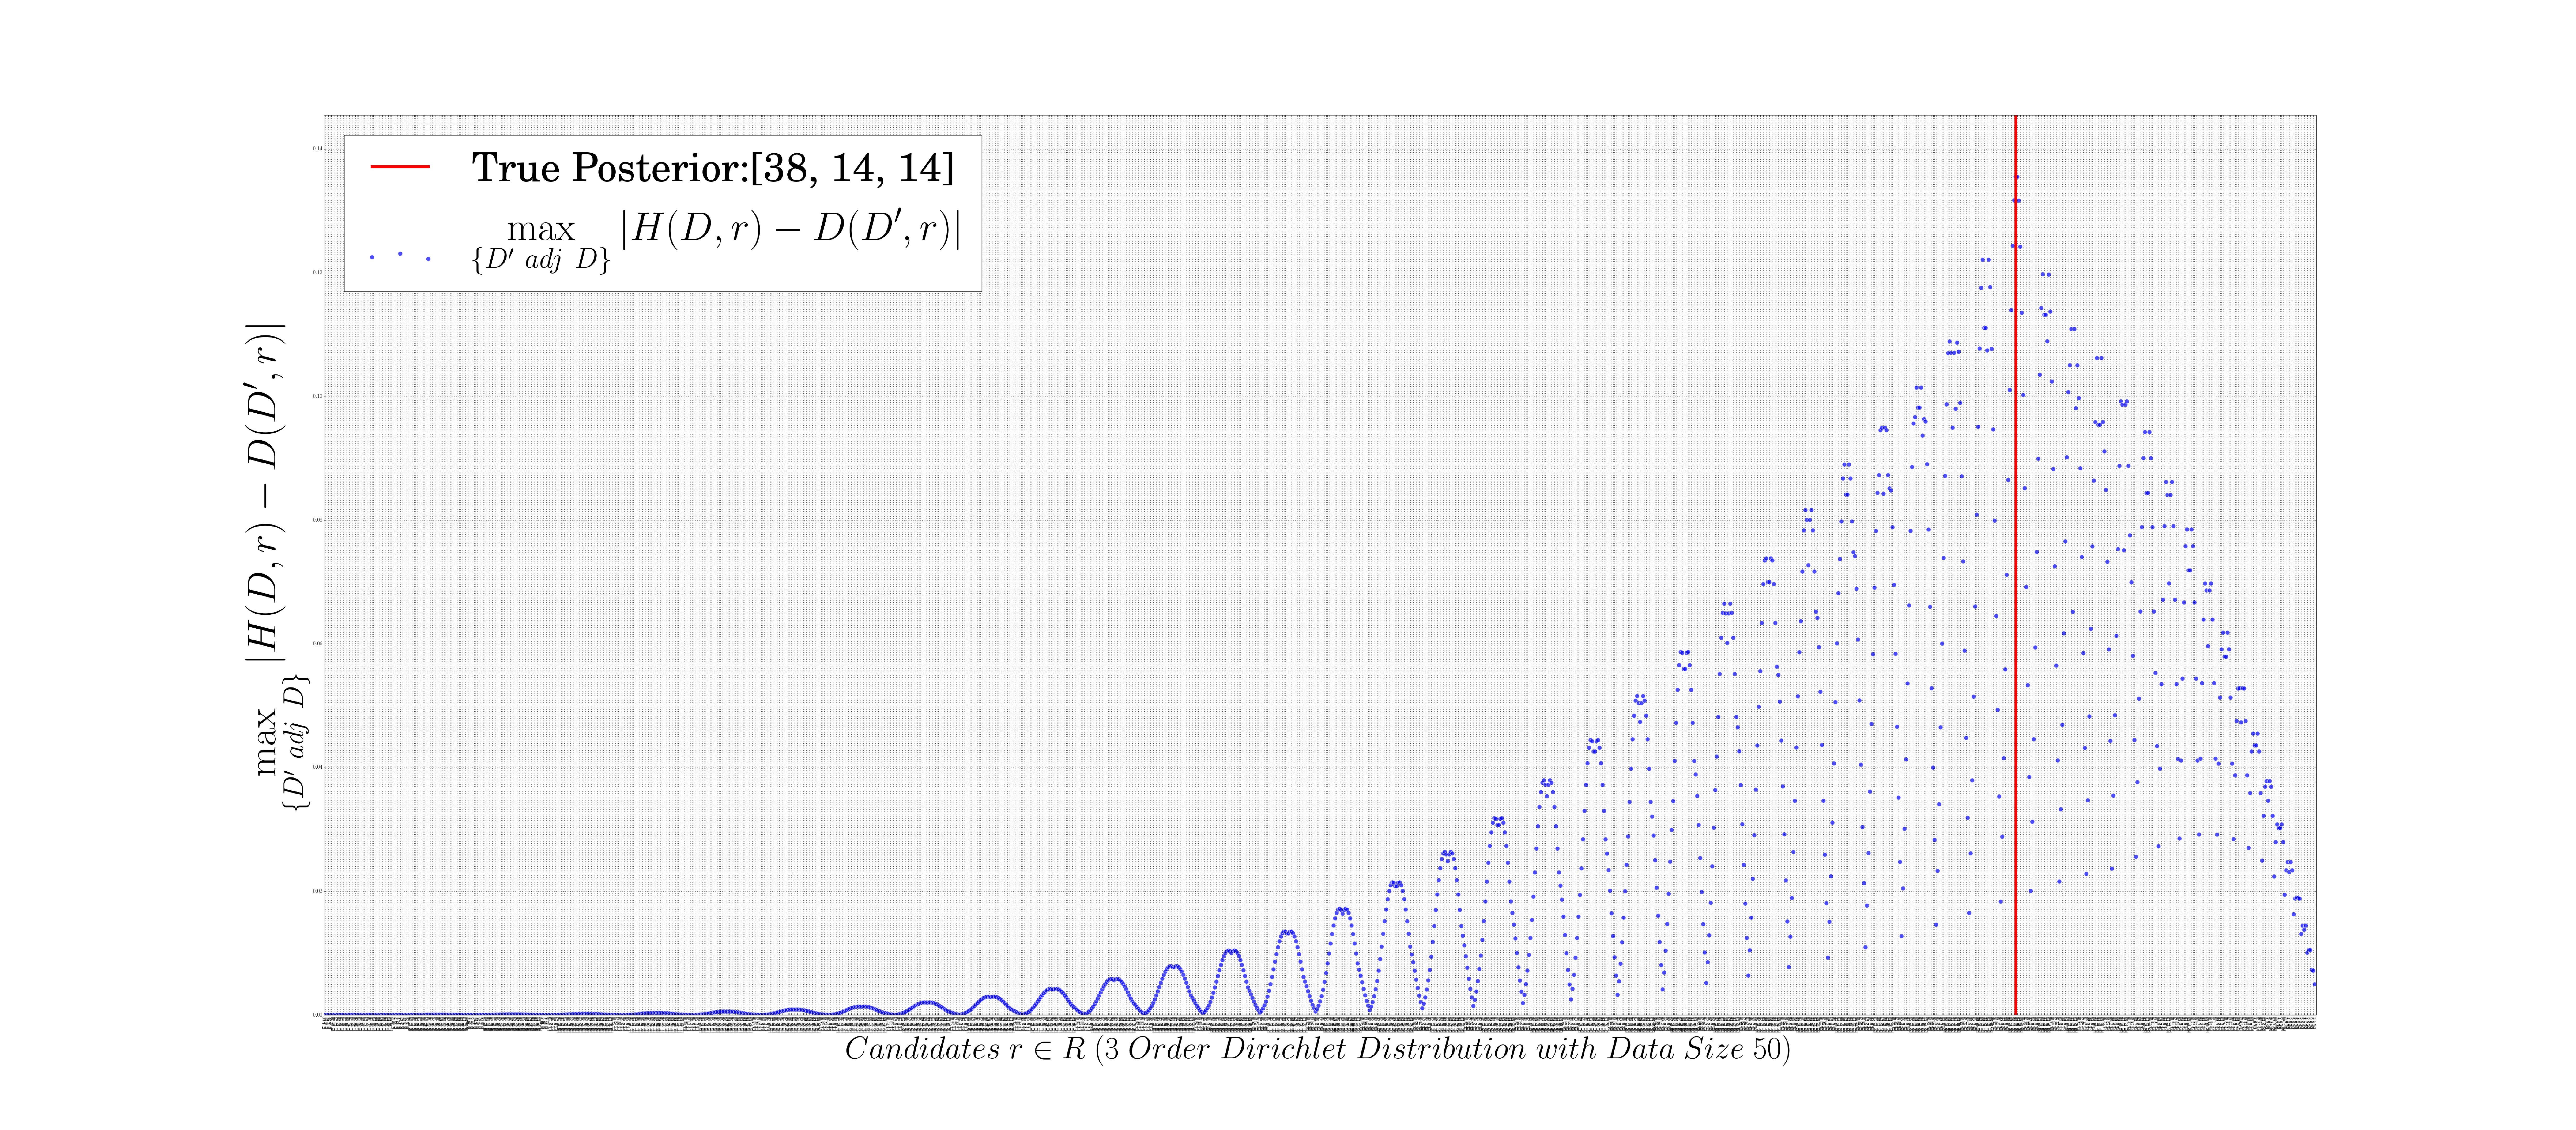
\includegraphics[width=0.48\textwidth]{efficiency}
\caption{Experimental Results for Finding the Local Sensitivity Efficiently}
\label{fig_efficiency}
\end{figure}

\subsection{Theoretical Results}

\begin{figure}[H]
\begin{center}
\centering
  \subfigure[2 dimensions with data size $600$]{
    \includegraphics[width=0.22\textwidth]{theory_2d.eps}
  \label{subfig_theory_2d}
  }
  \subfigure[3 dimensions with data size $600$]{
    \includegraphics[width=0.22\textwidth]{theory_3d.eps}
  \label{subfig_theory_3d}
  }
\caption{The theory probabilities of candidates in three mechanisms, with balanced data set and parameters $\epsilon = 1.0$ and $\delta = 10^{-8}$ }
\label{fig_theory}
\end{center}
\end{figure}
In Fig. \ref{fig_theory} we plot on the x-axis the Hellinger distance from the true posterior and on the y-axis the theoretical probabilities of outputting the candidates with that distance under the different mechanisms. We consider \emph{balanced} data sets, which means that in the Beta-Binomial model (Figure \ref{subfig_theory_2d}) the datasets will consist of 50\% 1s and the rest 0s, while for the
Dirichelet-Multinomial (Figure  \ref{subfig_theory_3d})
the data will be split in the $k=3$ bins with perecentages of: 33\%, 33\% and 34\% in 3 dimensionality. Same concept in 4 dimensionality.

In Fig. \ref{fig_theory}, candidates of smaller distance from true posterior can be outputted by $\hexpmech$ (in blue line) with larger probability than by baseline Laplace mechanism (in green line). This means $\hexpmech$ can produce good results with larger probability than baseline mechanism. However, the improved Laplace mechanism represented by red line can produce good results with probability higher than $\hexpmech$. It outperforms $\hexpmech$.


\subsection{Experimental Results}
\label{subsec_vs_variables}

In this section, we evaluate the accuracy of the mechanisms defined in
Section (\ref{sec_mechs}) w.r.t. four variables, including data size, dimensions,
data variance, prior distribution, and some combinations thereof.
Every plot is an average over 1000 runs. In all the experiments we set
$\epsilon = 1.0$, and $\delta = 10^{-8}$.

\noindent In the following some of the plots show
mean error as a function of the datasize while one
is a whiskers-plot where the y-axis shows the average
accuracy (or equivalently, the error) of the mechanisms, and the x-axis, instead shows
different balanced priors used. The boxes extend from the lower to the upper quartile values
of the data, with a line at the median. A notch on the box around the
median is also drawn to give a rough guide to the significance of
difference of medians; The whiskers extend from the box to show the
range of the data. A blue box in the plots represents our newly
designed exponential mechanism's behavior-- where the sensitivity is calibrated
w.r.t Hellinger distance-- while the yellow box next to
it represents the performance of a variation of the basic Laplace
mechanism presented in Section (\ref{subsec_baselines}) with the same
settings: that is $\epsilon, \delta$, data, prior. The variation
considered performs a postprocessing on the released parameters so
that they are consistent. For instance when the sum of the noised
parameters is greater than $n$ we will truncate them so that they sum
up to $n$.

\paragraph{Increasing data size with balanced datasets}
\label{subsubsec_vs_datasize}

\begin{figure}[H]
\begin{center}
\centering
    \includegraphics[width=0.4\textwidth]{sampling_2d.eps}
\caption{Increasing data size with prior $\betad(1,1)$, balanced datasets and parameters $\epsilon = 1.0$ and $\delta = 10^{-8}$}
\label{fig_vs_datasize_2d}
\end{center}
\end{figure}

\begin{figure}[ht]
\begin{center}
\centering
     \includegraphics[width=0.4\textwidth]{sampling_3d.eps}   
\caption{Increasing data size with $\dirichlet(1,1,1)$ prior distribution, balanced datasets and parameters $\epsilon = 1.0$ and $\delta = 10^{-8}$}
\label{fig_vs_datasize_3d}
\end{center}
\end{figure}

\begin{figure}[ht]
\begin{center}
\centering
     \includegraphics[width=0.4\textwidth]{sampling_4d.eps}    
\caption{Increasing data size with $\dirichlet(1,1,1,1)$ prior distribution, Unbalanced datasets and parameters $\epsilon = 1.0$ and $\delta = 10^{-8}$}
\label{fig_vs_datasize_4d}
\end{center}
\end{figure}

In Figures \ref{fig_vs_datasize_2d}, \ref{fig_vs_datasize_3d} and \ref{fig_vs_datasize_4d} we still consider \emph{balanced} data sets
of observations. The results show that when the data size increases, the average errors of
$\hexpmech$, Laplace mechanism and decrease. For small datasets,
i.e with size less $300$ in the case of Beta-Binomial models,
both the baseline Laplace mechanisms and improved Laplace mechanism outperform $\hexpmech$.
But for bigger data sets, that is, bigger than $300$, or as in Figure \ref{fig_vs_datasize_2d} where
we considered data sets of the order of 15 thousands elements,
the $\hexpmech$ outperforms the baseline Laplace mechanism, and asymptotically approaches the improved Laplace mechanism.
Similar experimental tendencies were obtained for the Dirichlet-multinomial model (Figure \ref{fig_vs_datasize_3d} and \ref{fig_vs_datasize_4d}).




\paragraph{Fixed dataset varying balanced priors}
\label{subsubsec_vs_prior}
In Figure \ref{fig_vs_prior}, we fix the data set to be $(50,50)$, and the parameters the same as before: $\epsilon = 1.0$ and $\delta = 10^{-8}$ . We studied the accuracy under different priors, where the priors considered  are also balanced.
Similar to the plots above, Figure \ref{fig_vs_prior} shows that in the beginning the baseline Laplace mechanism and improved Laplace mechanism performs better but the baseline approach is outperformed after a while, and very close to the improved Laplace mechanism.
\begin{figure}[H]
\centering
\includegraphics[width=0.48\textwidth]{sampling_prior.eps}
\caption{Observed data set is: $(50,50)$, varying balanced priors}
\label{fig_vs_prior}
\end{figure}

\subsection{Experiment Evaluations on Privacy Loss}
\label{subsec_experiment_privacy}
In order to see our privacy behavior, we study the accurate epsilon under concrete cases in this section. The $(\epsilon, \delta)$ - differential privacy we proved in Sec. \ref{subsec_hexpmech} is just an upper bound, we concrete $\epsilon$ should be smaller than upper bound in our exponential mechanism. We calculate the concrete privacy value in following ways wrt. the data size, and obtain plots in Fig. \ref{fig_privacy}.

\begin{figure}
\begin{center}
\centering
  \subfigure[data size range from 50 to 100]{
    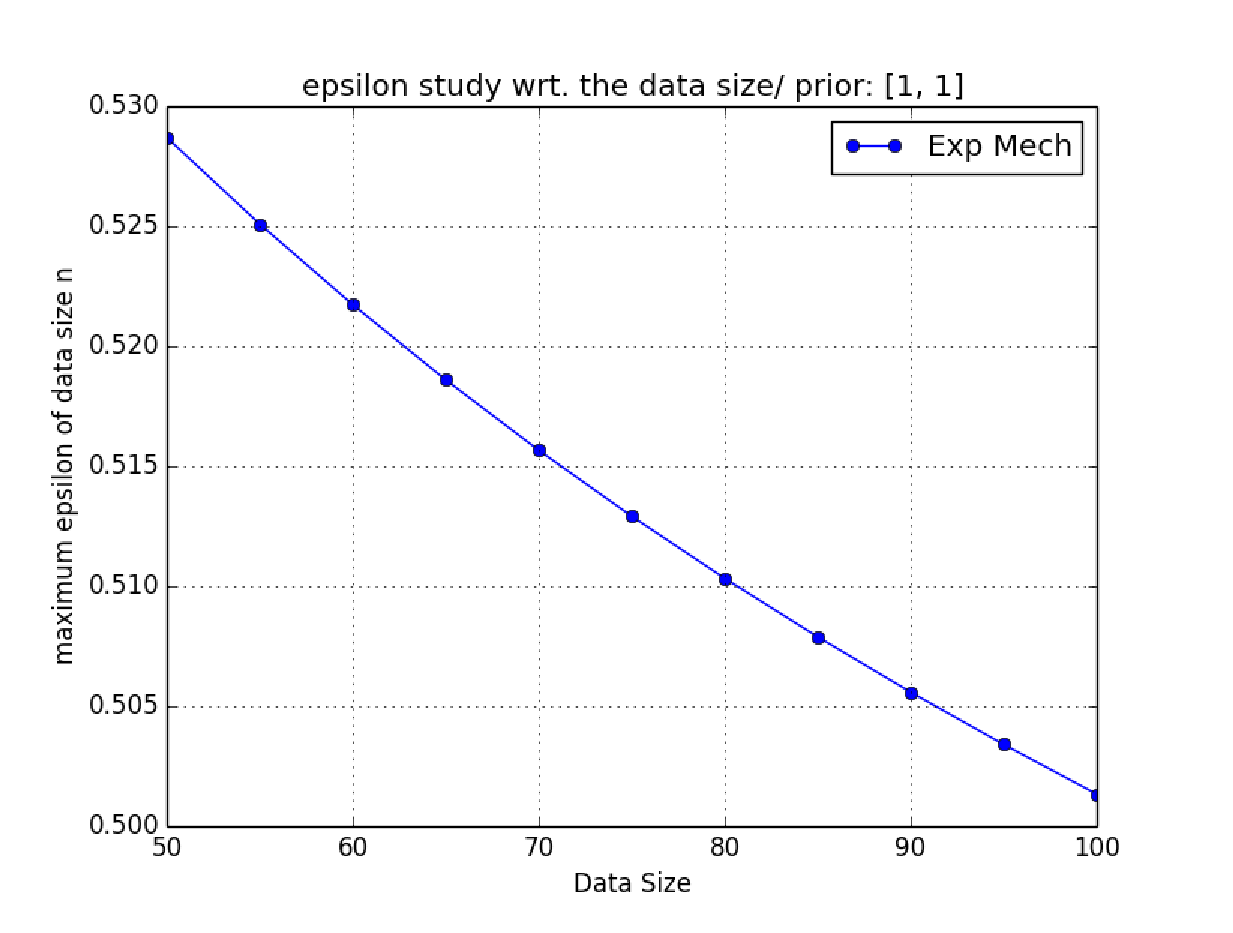
\includegraphics[width=0.23\textwidth]{global_epsilon_size50to100.eps}}
  \subfigure[data size range from 100 to 200]{
    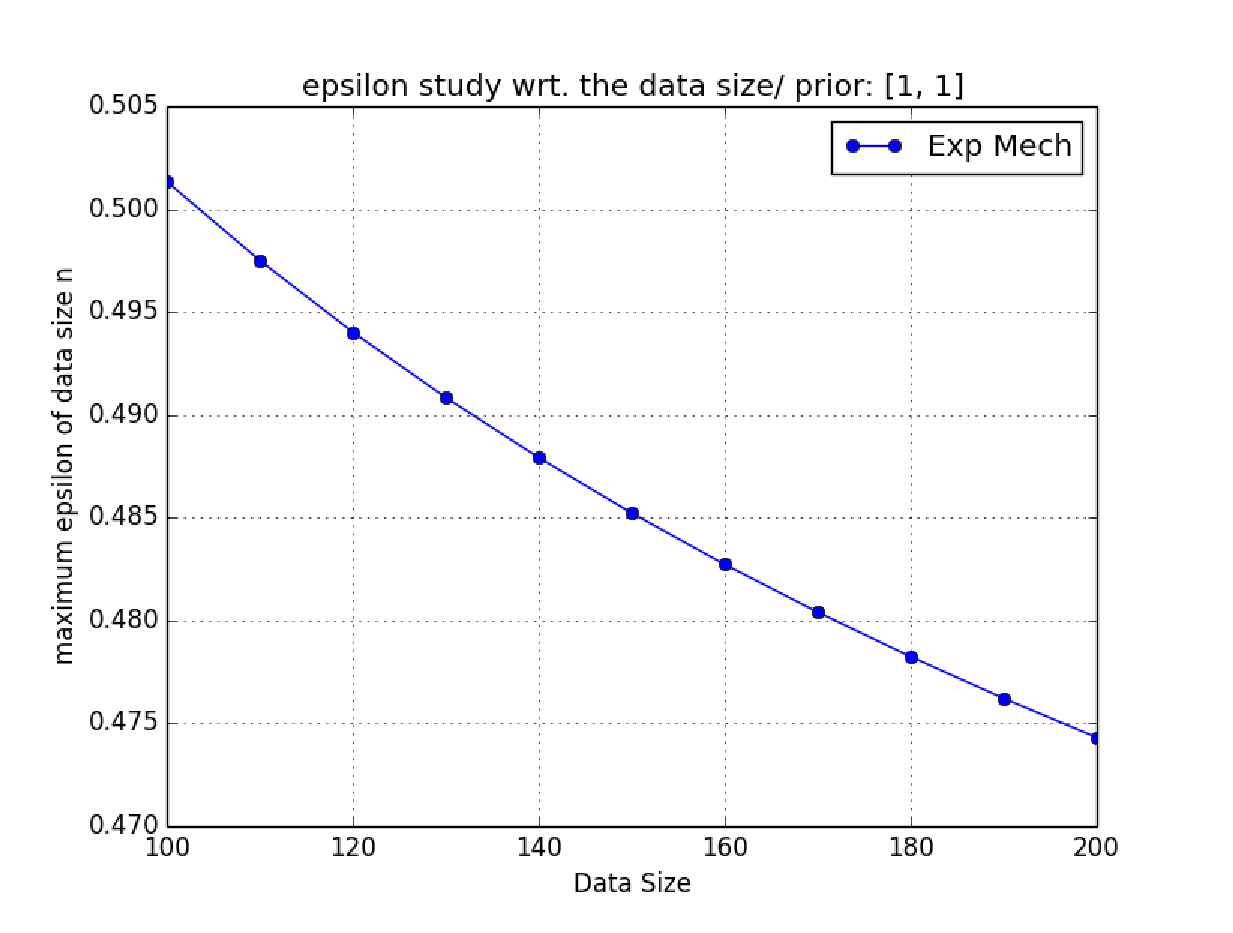
\includegraphics[width=0.23\textwidth]{global_epsilon_size100to200.eps}} 
  \subfigure[data size range from 200 to 500]{
    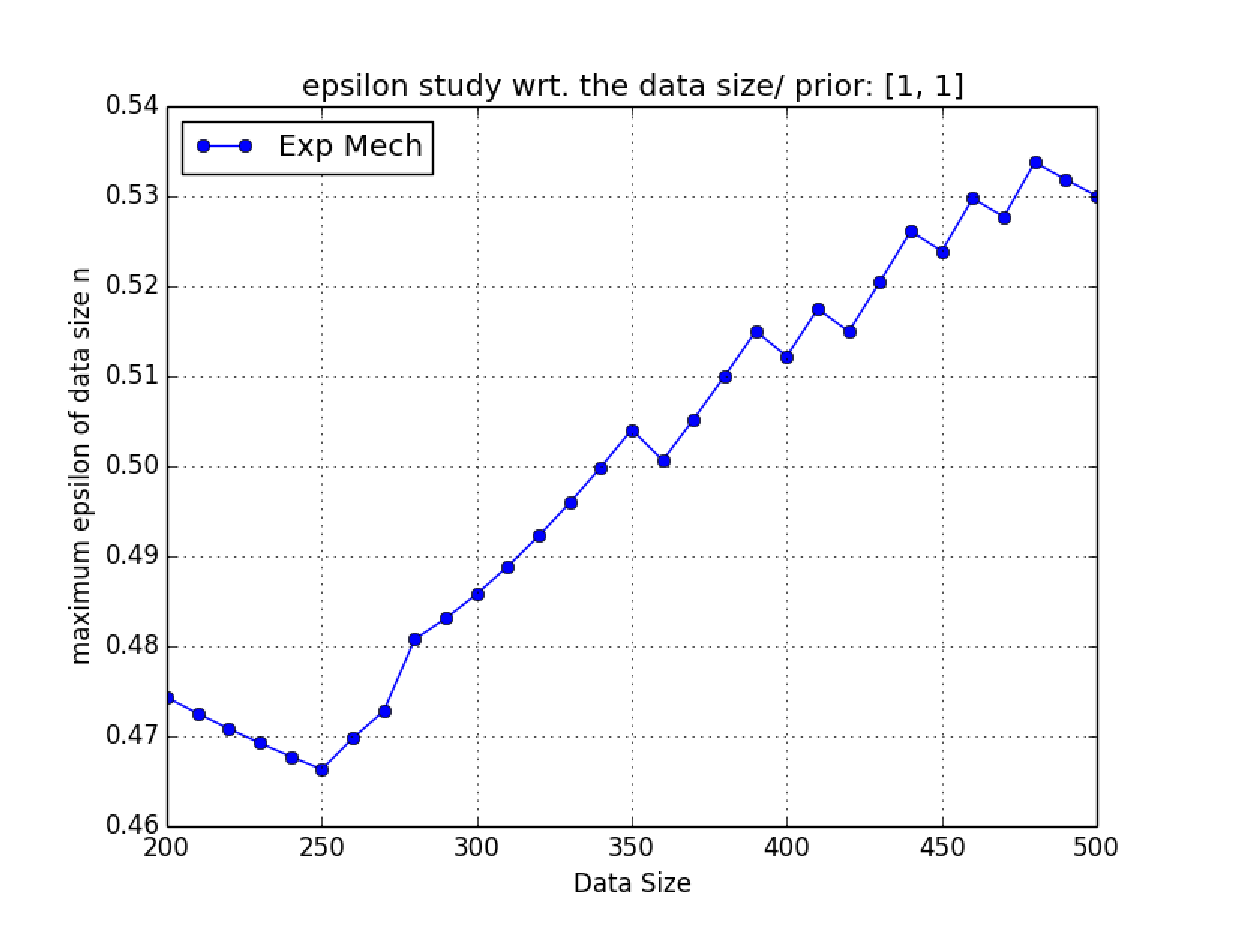
\includegraphics[width=0.23\textwidth]{global_epsilon_size200to500.eps}} 
  \subfigure[data size range from 500 to 1000]{
    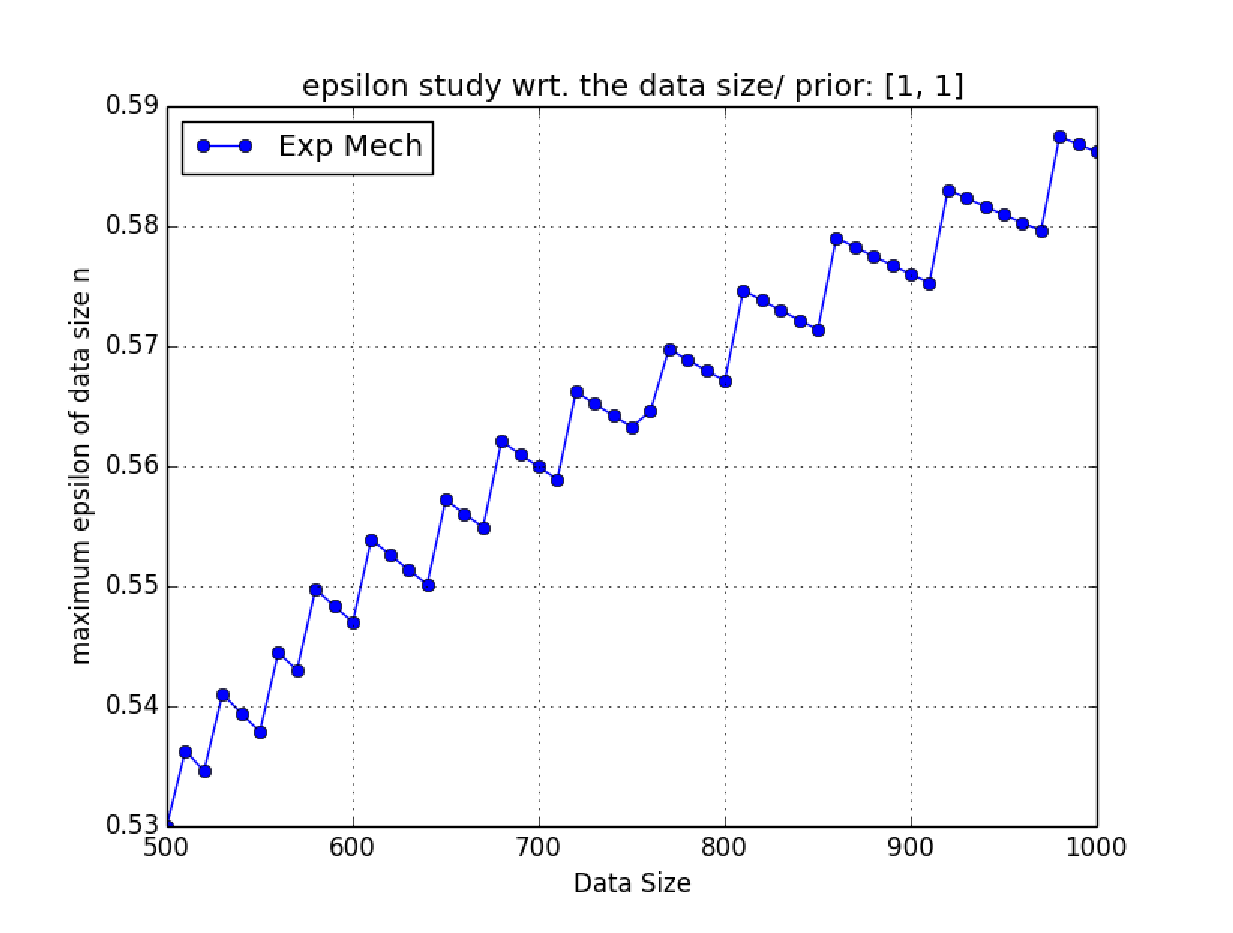
\includegraphics[width=0.23\textwidth]{global_epsilon_size500to1000.eps}} 
\caption{Concrete privacy calculation under settings that: prior distribution:$[1,1]$, $\epsilon = 1.0$, $\delta = 0.0005$ and observed data are uniformly distributed}
\label{fig_privacy}
\end{center}
\end{figure}

$\epsilon = 1.0$ is a privacy upper bound, we can observe that the concrete $\epsilon$ values are smaller than the upper bound. That is to say, we achieved a higher privacy level than expected. In next step, we are going to improve the accuracy using this property.


\bibliographystyle{ACM-Reference-Format}
\bibliography{bayesian.bib}

\end{document}

